\section{Program Generation}
\label{sec:related-work-generation}

The generation of artificial programs is a broad field with a wide range of applications. This section categorises the literature the use cases that are relevant to this thesis: program generation for performance characterisation, and program generation for compiler validation.

\subsection{Performance Characterisation}
\label{subsec:training-with-synthetic-benchmarks}

% Toffola, L. D., Pradel, M., & Gross, T. R. (2018). Synthesizing programs that expose performance bottlenecks. In CGO.
\todo[inline]{Synthesis to expose performance bottlenecks~\cite{Toffola2018}.}

\emph{GENESIS}~\cite{Chiu2015} is a language for generating synthetic training programs. The essence of the approach is to construct a probabilistic grammar with embedded semantic actions that defines a language of possible programs. New programs may be created by sampling the grammar and, through setting probabilities on the grammar productions, the sampling is biased towards producing programs from one part of the space or another. This technique is potentially completely general, since a grammar can theoretically be constructed to match any desired program domain. However, despite being theoretically possible, it is not easy to construct grammars which are both suitably general and also produce programs that are in any way similar to human written programs. It has been shown to be successful over a highly restricted space of stencil benchmarks with little control flow or program variability~\cite{Garvey2015b,Falch2015,Cummins2015}. But, it is not clear how much effort it will take, or even if it is possible for human experts to define grammars capable of producing human like programs in more complex domains. By contrast, learning from a corpus provides \emph{general-purpose} program generation over unknown domains, in which the statistical distribution of generated programs is automatically inferred from real world code.

% Joshi, A. M., Eeckhout, L., & John, L. K. (2008). The Return of Synthetic Benchmarks. In SPEC Benchmark Workshop.
\todo[inline]{Synthetic benchmarks~\cite{Joshi}.}

% Brockschmidt, M., Allamanis, M., Gaunt, A. L., & Polozov, O. (2018). Generative Code Modeling with Graphs. Retrieved from http://arxiv.org/abs/1805.08490
\todo[inline]{Generative code modelling with graphs~\cite{Brockschmidt2018}.}

The use of synthetic benchmarks for providing empirical performance
evaluations dates back to as early as 1974~\cite{Curnow1976}. The
\emph{automatic generation} of such synthetic benchmarks is a more
recent innovation, serving the purpose initially of stress-testing
increasingly complex software systems for behaviour validation and
automatic bug detection~\cite{Verplaetse2000,Godefroid2008}. A range
of techniques have been developed for these purposes, ranging from
applying random mutations to a known dataset to generate test stimuli,
to so-called ``white-box fuzz testing'' which analyses program traces
to explore the space of a program's control flow. CSmith is one such
tool which generates randomised C source programs for the purpose of
automatically detecting compiler bugs~\cite{Yang2012}.

A method for the automatic generation of synthetic benchmarks for the
purpose of \emph{performance} tuning is presented
in~\cite{Chiu2015}. \citeauthor{Chiu2015} use template substitution
over a user-defined range of values to generate training programs with
a statistically controlled range of features. A Perl preprocessor
generates output source codes from an input description using a custom
input language Genesis. Genesis is more flexible than the system
presented in this thesis, supporting substitution of arbitrary
sources. The authors describe an application of their tool for
generating OpenCL stencil kernels, but do not report any performance
results.

\emph{GENESIS}~\cite{Chiu2015} is a language for generating synthetic training programs. Users annotate template programs with statistical distributions over features, which are instantiated to generate statistically controlled permutations of templates. Template based approaches provide domain-specific solutions for a constrained feature and program space, for example, generating permutations of Stencil codes~\cite{Garvey2015b,Cummins2015a}. Our approach provides \emph{general-purpose} program generation over unknown domains, in which the statistical distribution of generated programs is automatically inferred from real world code.

Random program generation is an effective method for software testing. Grammar-based \emph{fuzz testers} have been developed for C~\cite{Yang2012} and OpenCL~\cite{Lidbury2015a}. A mutation-based approach for the Java Virtual Machine is demonstrated in~\cite{Chena}. Goal-directed program generators have been used for a variety of domains, including generating linear transforms~\cite{Voronenko2009}, MapReduce programs~\cite{Smith}, and data structure implementations~\cite{Loncaric2016}. Program synthesis from input/output examples is used for simple algorithms in~\cite{Zaremba2015a}, string manipulation in~\cite{Gulwani2011}, and geometry constructions in~\cite{Gulwani2012}.

Machine learning has been applied to source code to aid software engineering. Naturalize employs techniques developed in the natural language processing domain to model coding conventions~\cite{Allamanis2014a}. JSNice leverages probabilistic graphical models to predict program properties such as identifier names for JavaScript~\cite{Raychev}.


%\subsection{Parallelism}
%
%Programming languages have taken a variety of approaches in adopting parallelism. In C, a threading model was retrofitted using the \textit{POSIX pthreads} standard~\cite{Sura2005}. \citeauthor{Boehm2005} contends this approach in~\cite{Boehm2005}, describing issues in which a compiler developed independently of threading issues cannot be guaranteed to produce correct code. These issues were circumvented in C++11 by the introduction of a concurrency model~\cite{Boehm2008}, based off the success of the Java memory model~\cite{Bash2015a}. C++ and Java are two of the most popular imperative programming languages, and in both cases, the languages specify memory models which guarantee sequential consistency across threads, subject to some restrictions. A dialect of the Java programming language, Titanium, extends the Java feature set, adding multidimensional arrays, immutable classes, and a PGAS programming model~\cite{Yelick1998}. In contrast, Deterministic Parallel Java adds a type and effect system to in order to provide a provably sound language core~\cite{Bocchino2009}.
%
%
%%
%%% \subsubsection{Limits of static analysis}
%%Sequential consistency in shared-memory parallel programming~\cite{Krishnamurthy1995,Shasha1988,Sura2005}. Sequential consistency and caches~\cite{Goodman}.
%%
%%Sequential consistency for Java incurs a 10\% slowdown~\cite{Sura2005}.
%%
%
%%
%%Parallelism in the modern functional languages: Haskell, Clojure and Erlang~\cite{Pierro2012}.
%%
%%Scala actors~\cite{Haller2009a}, and~\cite{Haller2012}.
%%
%%
%%\subsubsection{Library level parallelism} Optimising MapReduce for multi-core processors~\cite{Kaashoek2010}.
%%\todo{OpenMP, MPI}
%
%
%\subsubsection{Automatic parallelisation} The goal of automatic parallelisation is to transform arbitrary sequential code into parallelised code. This is a well studied subject, with the typical approach being to perform these code transformations at the compilation stage. In \citeauthor{Banerjee1993}'s thorough review~\cite{Banerjee1993} of the subject, they outline the key challenges of automatic parallelisation: determining whether sequential code can be legally transformed for parallel execution; and identifying the transformation which will provide the highest performance improvement for a given piece of code. Both challenges are hard to tackle. For the former, the difficulties lie in performing accurate analysis of code behaviour. Obtaining accurate dynamic dependency analysis at compile time is an unsolved problem, as is resolving pointers and points-to analysis~\cite{Atkin-granville2013, Hind2001,Ghiya2001}.
%
%The result of these challenges is that reliably performant, automatic parallelisation of arbitrary programs remains a far reaching goal; however, there are noteworthy variations on which have been able to achieve some measure of success. One such example is speculative parallelism, which circumvents the issue of having incomplete dependency information by speculatively executing code regions in parallel while performing dependency tests at runtime, with the possibility to fall back to ``safe'' sequential execution if correctness guarantees are not met~\cite{Prabhu2010,Trachsel2010}.  In~\cite{Jimborean2014}, \citeauthor{Jimborean2014} present a system which combines polyhedral transformations of user code with binary algorithmic skeleton implementations for speculative parallelisation, reporting speedups over sequential code of up to $15.62\times$ on a 24 core processor.
%
%Annotation-driven parallelism takes a similar approach. The user annotates their code to provide ``hints'' to the compiler, which can then perform parallelising transformations. A popular example of this is OpenMP, which uses compiler pragmas to mark code sections for parallel or vectorised execution~\cite{Dagum1998}. Previous work has demonstrated code generators for translating OpenMP to OpenCL~\cite{Grewe2013} and CUDA~\cite{Lee2009}. Again, annotation-driven parallelism suffers from placing a burden on the developer to identify the potential areas for parallelism, and lacks the structure that algorithmic skeletons provide.


%
%
%\subsubsection{Debugging}
%General purpose, platform-specific debuggers: Intel Debugger for Linux~\cite{Blair-chappell}.
%
%
%% \subsubsection{Debugging Parallel Frameworks and Libraries}
%
%Allinea DDT~\cite{K2010}, a scalable parallel debugger.
%
%TotalView~\cite{Cownie2000}, an OpenMP debugger.
%
%Jumbune~\cite{ImpetusTechnologies}, an open source debugger for Hadoop.
%
%The parallel pipeline library FlumeJava~\cite{Chambers2010} provides debugging support through regular tools using a sequential execution mode,r and routing of exceptions and output from remote workers back to a central host.
%
%
%% \subsubsection{Debugging GPGPU programs}
%
%CUDA-GDB~\cite{NVIDIA2016}, Intel OpenCL Debugger for Linux
%OS~\cite{IntelCorporation2016}.
%
%Oclgrind~\cite{Price2015}.
%
%GPUverify~\cite{Betts2012}.
%
%
%% \subsubsection{Debugging Algorithmic Skeletons}
%SkIE~\cite{Bacci1999} is based on a coordination language, but provides advanced features such as debugging tools, performance analysis, visualization, and graphical user interface. Instead of directly using the coordination language, programmers interact with a graphical tool, where parallel modules based on skeletons can be composed
%
%SKiPPER~\cite{Serot1999} supports sequential execution for debugging.
%
%
%\subsubsection{Profiling}
%Profiling sequential programs~\cite{Ball1994}.
%
%% \subsubsection{Profiling parallel programs}
%Profiling parallel programs using KOJAK~\cite{Mohr2003}.
%
%


%\subsection{Performance Benchmarking}
%
%Rodinia~\cite{Che2009,Che2010},
%NPB (SNU~\cite{Seo2011}),
%Parboil~\cite{Stratton2012},
%PolyBench~\cite{Grauer-Gray2012},
%SHOC~\cite{Danalis2010}.
%
%Evaluating GPGPU benchmarks~\cite{Ryoo2015}.
%
%Benchmarking parallel computing systems~\cite{Belli2015}.
%
%\subsubsection{Methodology} Use geometric mean for speedups~\cite{Fleming1986}. Statistical rigour\cite{Georges2007}. Execution times and variance~\cite{Box}.
%
%\subsection{Self-Tuning Software}
%



\todo[inline]{Integrate CGO'17 related work section}

Our work lies at the intersections of a number of areas: program generation, benchmark characterisation, and language modelling and learning from source code. There is no existing work which is similar to ours, in respect to learning from large corpuses of source code for benchmark generation.

\emph{GENESIS}~\cite{Chiu2015} is a language for generating synthetic training programs. Users annotate template programs with statistical distributions over features, which are instantiated to generate statistically controlled permutations of templates. Template based approaches provide domain-specific solutions for a constrained feature and program space, for example, generating permutations of Stencil codes~\cite{Garvey2015b,Cummins2015a}. Our approach provides \emph{general-purpose} program generation over unknown domains, in which the statistical distribution of generated programs is automatically inferred from real world code.

Random program generation is an effective method for software testing. Grammar-based \emph{fuzz testers} have been developed for C~\cite{Yang2012} and OpenCL~\cite{Lidbury2015a}. A mutation-based approach for the Java Virtual Machine is demonstrated in~\cite{Chena}. Goal-directed program generators have been used for a variety of domains, including generating linear transforms~\cite{Voronenko2009}, MapReduce programs~\cite{Smith}, and data structure implementations~\cite{Loncaric2016}. Program synthesis from input/output examples is used for simple algorithms in~\cite{Zaremba2015a}, string manipulation in~\cite{Gulwani2011}, and geometry constructions in~\cite{Gulwani2012}.

Machine learning has been applied to source code to aid software engineering. Naturalize employs techniques developed in the natural language processing domain to model coding conventions~\cite{Allamanis2014a}. JSNice leverages probabilistic graphical models to predict program properties such as identifier names for JavaScript~\cite{Raychev}.

There is an increasing interest in mining source code repositories at large scale~\cite{Allamanis2013a,White2015a,Bird2009}. Previous studies have involved data mining of GitHub to analyse software engineering practices~\cite{Wu2014,Guzman2014,Baishakhi2014a,Vasilescu2015}, for example code generation~\cite{Zhang2015a}, code summarisation~\cite{Allamanis2016}, comment generation~\cite{Wong2013}, and code completion~\cite{Raychev2014}. However, no work so far has exploited mined source code for benchmark generation. This work is the first to do so.

Generative models for video~\cite{Srivastava2015}.

%% Jozefowicz, R., Vinyals, O., Schuster, M., Shazeer, N., & Wu, Y. (2016). Exploring the Limits of Language Modeling. arXiv:1602.02410. Retrieved from http://arxiv.org/abs/1602.02410%5Cnhttp://www.arxiv.org/pdf/1602.02410.pdf
Limits of language modelling~\cite{Jozefowicz2016a}.

%% Sutskever, I., Vinyals, O., & Le, Q. V. (2014). Sequence to Sequence Learning with Neural Networks. In NIPS.
Sequence to sequence learning, NIPS paper~\cite{Sutskever2014}.


\subsection{Compiler Validation}

Compilers are a fundamental trusted technology, and their correctness is critical. Errors in compilers can introduce security vulnerabilities and catastrophic runtime failures. Therefore, verifying the behaviour of a compiler is of utmost importance.

The complexity of optimizing compilers and programming languages renders formal verification of the entire compiler prohibitively expensive. Efforts have been made in this directory, for example CompCert~\cite{Leroy2013}, a formally verified compiler for the C programming language, but this comes at the cost of supporting only a subset of the language features and with lower performance compared to GCC. Still, even CompCert is not fully verified, and errors have been discovered in the unverified components of it~\cite{Yang2011}.

Because of the difficulties of \emph{verification}, compilers developers turn to \emph{validation}, in which the behaviour of a compiler is validated using a set of input test cases (i.e. programs). For each test case, the expected outcome (determined by the specification of the compiler) is compared against the observed outcome to verify that the compiler conforms to the specification, for those inputs. However, the absence of errors for does not prove that the compiler is free from errors unless all possible inputs are tested exhaustively, and the input space for compilers is huge. As such, hand designed suites of test programs, while important, are inadequate for covering such a large space and will not touch all parts of the compiler.

The random generation of programs to test compilers is a well established approach to the compiler validation problem. Initial approaches  based on a formal specification of the programming language syntax and grammar.

Prior approaches are surveyed in~\cite{Kossatchev2005,Boujarwah1997} and empirically contrasted in~\cite{Chen2014a}. The main question of interest is in how to efficiently generate codes which trigger bugs. There are two main approaches: \emph{program generation}, where inputs are synthesised from scratch; and \emph{program mutation}, where existing codes are modified so as to identify anomalous behaviour.

\begin{figure}
	\centering
	\subfloat[][Expected outcome-based test case generation and evaluation]{%
		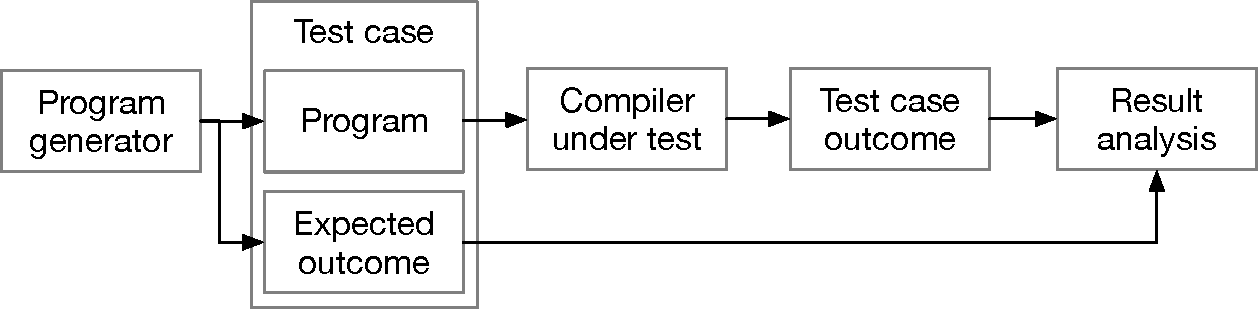
\includegraphics[width=.8\columnwidth]{img/oracle-generator}%
		\label{fig:test-case-generators-oracle}%
	}%
	\\*
	\subfloat[][Differential test case generation and evaluation]{%
		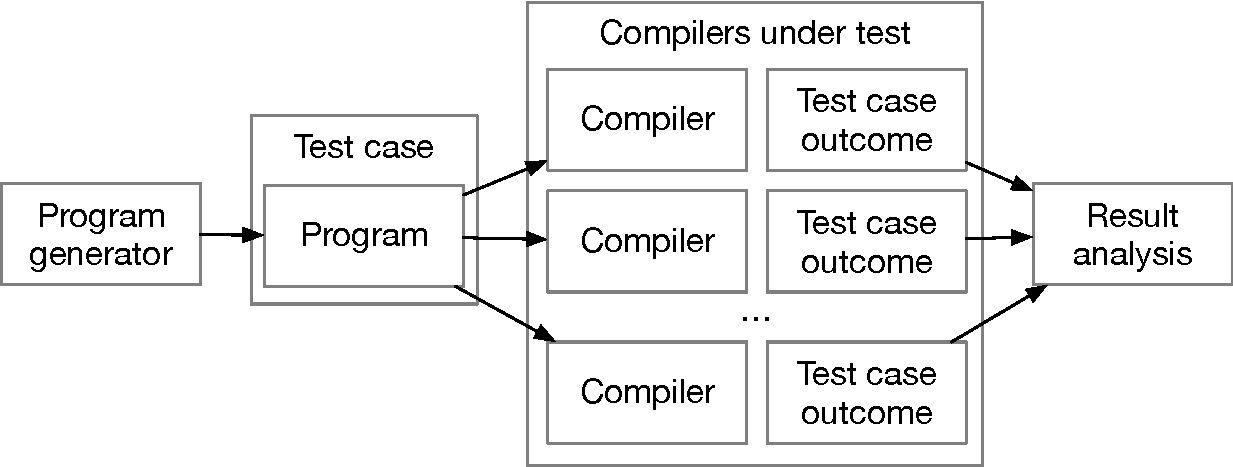
\includegraphics[width=.8\columnwidth]{img/difftest-generator}%
		\label{fig:test-case-generators-difftest}%
	}%
	\caption[Generating and evaluating compiler test cases]{%
		Two approaches to addressing the \emph{compiler validation} problem through test case generation. In~\protect\subref{fig:test-case-generators-oracle}, a test case comprises a program and its expected outcome. In~\protect\subref{fig:test-case-generators-difftest}, only a program is required, and the expected outcome is determined by majority voting on the observed outcomes across multiple compilers.%
	}%
	\label{fig:test-case-generators}
\end{figure}

Goal-directed program generators have been used for a variety of domains, including 
% Voronenko, Y., De Mesmay, F., & Püschel, M. (2009). Computer Generation of General Size Linear Transform Libraries. In CGO. IEEE. https://doi.org/10.1109/CGO.2009.33
generating linear transforms~\cite{Voronenko2009},
% Smith, C. (2016). MapReduce Program Synthesis. In PLDI.
MapReduce programs~\cite{Smith},
% Loncaric, C., Emina, T., & Ernst, M. D. (2016). Fast Synthesis of Fast Collections. In PLDI.
and data structure implementations~\cite{Loncaric2016}.

% PROBABILISTIC PROGRAMMING

% Bielik, P., Raychev, V., & Vechev, M. (2016). PHOG: Probabilistic Model for Code. In ICML. https://doi.org/10.1126/science.7.179.764
\todo[inline]{Probabilistic model for code~\cite{Bielik2016}.}

% Gaunt, A. L., Kushman, N., Brockschmidt, M., Kohli, P., Tarlow, D., Singh, R., & Taylor, J. (2016). TerpreT: A Probabilistic Programming Language for Program Induction. ArXiv:1608.04428.
\todo[inline]{Probabilistic programming~\cite{Gaunt2016}.}

% Liu, X., Li, X., Prajapati, R., & Wu, D. (2019). DeepFuzz: Automatic Generation of Syntax Valid C Programs for Fuzz Testing. In AAAI.
\todo[inline]{DeepFuzz~\cite{Liu2019}.}

% Nasrabadi, M. Z., Parsa, S., & Kalaee, A. (2018). Neural Fuzzing: A Neural Approach to Generate Test Data for File Format Fuzzing. ArXiv:1812.09961. Retrieved from https://arxiv.org/pdf/1812.09961.pdf
\todo[inline]{Fuzzing file formats~\cite{Nasrabadi}.}

\subsubsection{Differential Testing}

Differential testing accelerates testing by enabling multiple compilers to be tested at once. It is less sound than an oracle approach (since we don't have a golden standard for expected outcome), but in practise no work in the literature has reported false positives as a result. False negatives are unlikely, but not detectable ofc.

In the foundational work on differential testing for compilers, McKeeman \emph{et al.\ }present generators capable of enumerating programs of a range of qualities, from random ASCII sequences to C model conforming programs~\cite{McKeeman1998}. Subsequent works have presented increasingly complex generators which improve in some metric of interest, generally expressiveness or probability of correctness. CSmith~\cite{Yang2011} is a widely known and effective generator which enumerates programs by pairing infrequently combined language features. In doing so, it produces correct programs with clearly defined behaviour but very unlikely functionality, increasing the chances of triggering a bug. Achieving this required extensive engineering work, most of it not portable across languages, and ignoring some language features. Subsequent generators influenced by CSmith, like Orange3~\cite{Nagai2013}, focus on features and bug types beyond the scope of CSmith, arithmetic bugs in the case of Orange3. Glade~\cite{Bastani2017} derives a grammar from a corpus of example programs. The derived grammar is enumerated to produce new programs, though unlike our approach, no distribution is learned over the grammar; program enumeration is uniformly random.

Random program generation is an effective method for software testing. Grammar-based \emph{fuzz testers} have been developed for C~\cite{Yang2012} and OpenCL~\cite{Lidbury2015a}. Programs generated by grammar-based approaches are often  unlike real handwritten code, and are typically very large. As such, once a bug has been identified, test case reduction~\cite{Regehr2012a} is required to minimise the size of the program and isolate the code of interest.

% She, D., Pei, K., Epstein, D., Yang, J., Ray, B., & Jana, S. (2018). NEUZZ: Efficient Fuzzing with Neural Program Learning. ArXiv:1807.05620.
\todo[inline]{Fuzzing through ML~\cite{She2018}.}

% Mathis, B., Kampmann, A., Gopinath, R., Höschele, M., Mera, M., & Zeller, A. (2019). Parser-Directed Fuzzing. In PLDI.
\todo[inline]{PLDI'19 fuzzing paper~\cite{Mathis2019}.}

There is an increasing interest in applying machine learning to software
testing. Most similar to our work is Learn\&fuzz~\cite{Godefroid2017}, in which
an LSTM network is trained over a corpus of PDF files to generate test inputs
for the Microsoft Edge renderer, yielding one bug. Unlike compiler testing, PDF
test cases require no inputs and no pre-processing of the training corpus.
Skyfire~\cite{Wang2017c} learns a probabilistic context-sensitive grammar over a
corpus of programs to generate input seeds for mutation testing. The generated
seeds are shown to improve the code coverage of AFL~\cite{Zalewski} when fuzzing
XSLT and XML engines, though the seeds are not directly used as test cases.


\subsubsection{Program Mutation}

Equivalence Modulo Inputs (EMI) testing~\cite{Le2013a,Sun2016a} follows a different approach to test case generation. Starting with existing code, it inserts or deletes statements that will not be executed, so functionality should remain the same. If it is affected, it is due to a compiler bug. While a powerful technique able to find hard to detect bugs, it relies on having a very large number of programs to mutate. As such, it still requires an external code generator. Similarly to CSmith, EMI favours very long test programs. LangFuzz~\cite{Holler2012} also uses mutation but does this by inserting code segments which have previously exposed bugs. This increases the chances of discovering vulnerabilities in scripting language engines. Skeletal program enumeration~\cite{Zhang2017a} again works by transforming existing code. It identifies algorithmic patterns in short pieces of code and enumerates all the possible permutations of variable usage. Compared to all these, our fuzzing approach is low cost, easy to develop, portable, capable of detecting a wide range of errors, and focusing by design on bugs that are more likely to be encountered in a production scenario.

A mutation-based approach for differential testing the Java Virtual Machine is demonstrated in~\cite{Chena}.